

%% NJCTL: PSI AP Physics C
%%----------------------------------------


%% Universal Gravity
%%----------------------------------------
\element{njctl}{
\begin{question}{gravity-q01}
    Who determined the value of the gravitational constant ($G$)?
    \begin{multicols}{2}
    \begin{choices}
        \wrongchoice{Newton}
        \wrongchoice{Galileo}
        \wrongchoice{Einstein}
        \wrongchoice{Schr\"{o}dinger}
      \correctchoice{Cavendish}
        %% Added by jphafner
        \wrongchoice{Hooke}
    \end{choices}
    \end{multicols}
\end{question}
}

\element{njctl}{
\begin{question}{gravity-q02}
    Who came up with the law for Universal Gravitation?
    \begin{multicols}{2}
    \begin{choices}
      \correctchoice{Newton}
        \wrongchoice{Galileo}
        \wrongchoice{Einstein}
        \wrongchoice{Schr\"{o}dinger}
        \wrongchoice{Cavendish}
        %% Added by jphafner
        \wrongchoice{Hooke}
    \end{choices}
    \end{multicols}
\end{question}
}

\element{njctl}{
\begin{question}{gravity-q03}
    Two large objects of equal mass $m$ are separated by a distance $r$ and exert a gravitational pull of magnitude $F$.
    If the distance between the two objects is reduced to $r/4$,
        what is the new gravitational force acting on each object?
    \begin{multicols}{3}
    \begin{choices}
        \wrongchoice{$\dfrac{F}{2}$}
        \wrongchoice{$\dfrac{F}{4}$}
        \wrongchoice{$\dfrac{F}{16}$}
        \wrongchoice{$4F$}
      \correctchoice{$16F$}
    \end{choices}
    \end{multicols}
\end{question}
}

\element{njctl}{
\begin{question}{gravity-q04}
    Two large objects of equal mass $m$ are separated by a distance $r$ and exert a gravitational pull of magnitude $F$.
    If the distance between the two objects is reduced to $r/4$,
        what is the new gravitational force acting on each object?
    \begin{multicols}{3}
    \begin{choices}
        \wrongchoice{$\dfrac{F}{2}$}
      \correctchoice{$\dfrac{F}{4}$}
        \wrongchoice{$\dfrac{F}{16}$}
        \wrongchoice{$4F$}
        \wrongchoice{$16F$}
    \end{choices}
    \end{multicols}
\end{question}
}

\element{njctl}{
\begin{question}{gravity-q05}
    A satellite is orbiting the Earth a distance $R_E$ above its surface.
    What is the acceleration due to gravity in this orbit?
    ($R_E$ is the radius of the earth)
    \begin{multicols}{3}
    \begin{choices}
      \correctchoice{\SI{2.45}{\meter\per\second\squared}}
        \wrongchoice{\SI{4.9}{\meter\per\second\squared}}
        \wrongchoice{\SI{9.8}{\meter\per\second\squared}}
        \wrongchoice{\SI{19.6}{\meter\per\second\squared}}
        \wrongchoice{\SI{39.2}{\meter\per\second\squared}}
    \end{choices}
    \end{multicols}
\end{question}
}

\element{njctl}{
\begin{question}{gravity-q06}
    A satellite is orbiting a planet a distance $R$ from its center and another satellite is orbiting at a distance $3R$ from its center.
    \begin{center}
    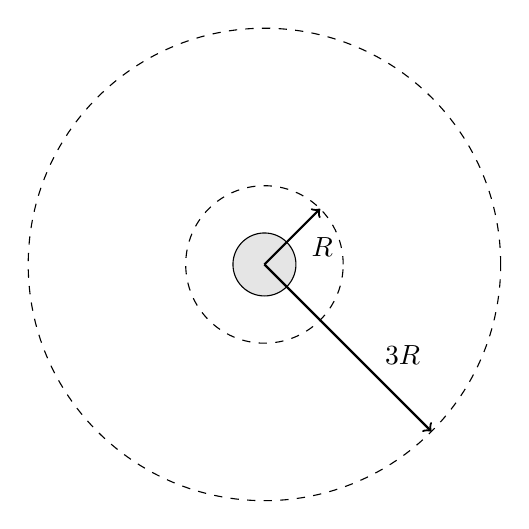
\begin{tikzpicture}
        %% Planet
        \draw[fill=white!90!black] (0,0) circle (0.4cm);
        %% Orbits
        \draw[dashed] (0,0) circle (3cm);
        \draw[thick,->] (0,0) -- (315:3) node[pos=0.66,anchor=south west] {$3R$};
        \draw[dashed] (0,0) circle (1cm);
        \draw[thick,->] (0,0) -- (45:1) node[pos=0.66,anchor=north west] {$R$};
    \end{tikzpicture}
    \end{center}
    What is the relation between the accelerations due to gravity for each case?
    ($a_1$ is the acceleration a distance $R$ away from its center and $a_2$ is the acceleration due to gravity a distance $3R$ from its center)
    \begin{multicols}{3}
    \begin{choices}
      \correctchoice{$a_2 = \dfrac{a_1}{9}$}
        \wrongchoice{$a_2 = \dfrac{a_1}{3}$}
        \wrongchoice{$a_2 = a_1$}
        \wrongchoice{$a_2 = 3a_1$}
        \wrongchoice{$a_2 = 9a_1$}
    \end{choices}
    \end{multicols}
\end{question}
}

\element{njctl}{
\begin{question}{gravity-q07}
    Planet $\beta$ has 2 times the mass of the Earth and $1/2$ of the radius.
    The acceleration due to gravity at the surface is closest to:
    \begin{multicols}{3}
    \begin{choices}
        \wrongchoice{\SI{20}{\meter\per\second\squared}}
        \wrongchoice{\SI{40}{\meter\per\second\squared}}
      \correctchoice{\SI{80}{\meter\per\second\squared}}
        \wrongchoice{\SI{3}{\meter\per\second\squared}}
        \wrongchoice{\SI{5}{\meter\per\second\squared}}
    \end{choices}
    \end{multicols}
\end{question}
}

\element{njctl}{
\begin{question}{gravity-q08}
    Planet $\alpha$ has 5 times the mass of the Earth and 2 times the radius.
    The acceleration due to gravity at the surface of planet $\alpha$ is closest to:
    \begin{multicols}{3}
    \begin{choices}
        \wrongchoice{\SI{6.125}{\meter\per\second\squared}}
      \correctchoice{\SI{12.5}{\meter\per\second\squared}}
        \wrongchoice{\SI{25}{\meter\per\second\squared}}
        \wrongchoice{\SI{10}{\meter\per\second\squared}}
        \wrongchoice{\SI{49}{\meter\per\second\squared}}
    \end{choices}
    \end{multicols}
\end{question}
}

\element{njctl}{
\begin{question}{gravity-q09}
    What is the weight of an object that has a mass of \SI{10}{\kilo\gram} on the surface of the Earth?
    \begin{multicols}{3}
    \begin{choices}
        \wrongchoice{\SI{49}{\newton}}
        \wrongchoice{\SI{64}{\newton}}
        \wrongchoice{\SI{86}{\newton}}
      \correctchoice{\SI{98}{\newton}}
        \wrongchoice{\SI{110}{\newton}}
    \end{choices}
    \end{multicols}
\end{question}
}

\element{njctl}{
\begin{question}{gravity-q10}
    A mass of \SI{10}{\kilo\gram} is placed on the surface of Mars.
    What is its mass?
    (The acceleration due to gravity on Mars is \SI{3.7}{\meter\per\second\squared})
    \begin{multicols}{3}
    \begin{choices}
        \wrongchoice{\SI{0.37}{\kilo\gram}}
        \wrongchoice{\SI{3.7}{\kilo\gram}}
        \wrongchoice{\SI{37}{\kilo\gram}}
      \correctchoice{\SI{10}{\kilo\gram}}
        \wrongchoice{\SI{100}{\kilo\gram}}
    \end{choices}
    \end{multicols}
\end{question}
}

\element{njctl}{
\begin{question}{gravity-q11}
    A mass of \SI{10}{\kilo\gram} is placed on the surface of Mars.
    What is its weight?
    (The acceleration due to gravity on Mars is \SI{3.7}{\meter\per\second\squared})
    \begin{multicols}{3}
    \begin{choices}
        \wrongchoice{\SI{0.37}{\newton}}
        \wrongchoice{\SI{3.7}{\newton}}
      \correctchoice{\SI{37}{\newton}}
        \wrongchoice{\SI{10}{\newton}}
        \wrongchoice{\SI{100}{\newton}}
    \end{choices}
    \end{multicols}
\end{question}
}

\element{njctl}{
\begin{question}{gravity-q12}
    How much work is done by the force due to gravity when an object moves from the surface of the Earth to a height above its surface equal to its radius $R$?
    \begin{multicols}{2}
    \begin{choices}
        \wrongchoice{$W = \dfrac{GMm}{R}$}
      \correctchoice{$W = -\dfrac{GMm}{2R}$}
        \wrongchoice{$W = \dfrac{2GMm}{R}$}
        \wrongchoice{$W = \dfrac{GM}{R}$}
        \wrongchoice{$W = -\dfrac{GMm}{R}$}
    \end{choices}
    \end{multicols}
\end{question}
}

\element{njctl}{
\begin{question}{gravity-q13}
    What is the gravitational potential energy of an object located \SI{32 000}{\meter} above the Earth's Surface?
    \begin{multicols}{2}
    \begin{choices}
      \correctchoice{$U = -\dfrac{GMm}{\SI{32}{\kilo\meter} + R_E}$}
        \wrongchoice{$U = -\dfrac{GMm}{\SI{32 000}{\kilo\meter} + R_E}$}
        \wrongchoice{$U = -\dfrac{GMm}{R_E}$}
        \wrongchoice{$U = -\dfrac{GMm}{R_E - \SI{32}{\kilo\meter}}$}
        \wrongchoice{$U = -\dfrac{GM}{R_E}$}
    \end{choices}
    \end{multicols}
\end{question}
}

\element{njctl}{
\begin{question}{gravity-q14}
    As an object moves away from the surface of the Earth,
        the graph of the gravitational potential energy is:
    \begin{multicols}{2}
    \begin{choices}
        %% ANS is A
        \AMCboxDimensions{down=-1.5em}
        \correctchoice{
            \begin{tikzpicture}
                \begin{axis}[
                    axis y line=left,
                    axis x line=middle,
                    axis line style={->},
                    xlabel={radius},
                    xtick=\empty,
                    ylabel={energy},
                    ytick=\empty,
                    xmin=0,xmax=11,
                    ymin=-6,ymax=6,
                    width=0.95\columnwidth,
                    very thin,
                ]
                \addplot[line width=1pt,domain=0:10]{-5/x};
                \end{axis}
            \end{tikzpicture}
        }
        \wrongchoice{
            \begin{tikzpicture}
                \begin{axis}[
                    axis y line=left,
                    axis x line=middle,
                    axis line style={->},
                    xlabel={radius},
                    x label style={anchor=north east},
                    xtick=\empty,
                    ylabel={energy},
                    ytick=\empty,
                    xmin=0,xmax=11,
                    ymin=-6,ymax=6,
                    width=0.95\columnwidth,
                    very thin,
                ]
                \addplot[line width=1pt,domain=0:10]{-5+x};
                \end{axis}
            \end{tikzpicture}
        }
        \wrongchoice{
            \begin{tikzpicture}
                \begin{axis}[
                    axis y line=left,
                    axis x line=middle,
                    axis line style={->},
                    xlabel={radius},
                    x label style={anchor=north east},
                    xtick=\empty,
                    ylabel={energy},
                    ytick=\empty,
                    xmin=0,xmax=11,
                    ymin=-6,ymax=6,
                    width=0.95\columnwidth,
                    very thin,
                ]
                \addplot[line width=1pt,domain=0:10]{0.1*x*x};
                \end{axis}
            \end{tikzpicture}
        }
        \wrongchoice{
            \begin{tikzpicture}
                \begin{axis}[
                    axis y line=left,
                    axis x line=middle,
                    axis line style={->},
                    xlabel={radius},
                    x label style={anchor=north east},
                    xtick=\empty,
                    ylabel={energy},
                    ytick=\empty,
                    xmin=0,xmax=11,
                    ymin=-6,ymax=6,
                    width=0.95\columnwidth,
                    very thin,
                ]
                \addplot[line width=1pt,domain=0:10]{5/x};
                \end{axis}
            \end{tikzpicture}
        }
        \wrongchoice{
            \begin{tikzpicture}
                \begin{axis}[
                    axis y line=left,
                    axis x line=middle,
                    axis line style={->},
                    xlabel={radius},
                    x label style={anchor=north east},
                    xtick=\empty,
                    ylabel={energy},
                    ytick=\empty,
                    xmin=0,xmax=11,
                    ymin=-6,ymax=6,
                    width=0.95\columnwidth,
                    very thin,
                ]
                \addplot[line width=1pt,domain=0:10]{5-0.5*x};
                \end{axis}
            \end{tikzpicture}
        }
    \end{choices}
    \end{multicols}
\end{question}
}

\element{njctl}{
\begin{question}{gravity-q15}
    A rocket ship is sitting on the surface of a planet with a mass of \SI{e27}{\kilo\gram} and a radius of \SI{6.67e12}{\meter}.
    What is the planet's escape velocity?
    \begin{multicols}{2}
    \begin{choices}
        \wrongchoice{$\sqrt{200}\,\si{\meter\per\second}$}
        \wrongchoice{\SI{100}{\meter\per\second}}
      \correctchoice{$100\sqrt{2}\,\si{\meter\per\second}$}
        \wrongchoice{\SI{50}{\meter\per\second}}
        \wrongchoice{\SI{10}{\meter\per\second}}
    \end{choices}
    \end{multicols}
\end{question}
}

\element{njctl}{
\begin{question}{gravity-q16}
    There are two Planets, each with the same surface gravity,
        but Planet 1 has a greater radius and is less massive then Planet 2.
    Which of these planets has a greater escape velocity?
    \begin{choices}
        \wrongchoice{Planet 1}
      \correctchoice{Planet 2}
        \wrongchoice{Both have the same escape velocity because surface gravity is equal}
        \wrongchoice{Not enough information is given}
    \end{choices}
\end{question}
}

\element{njctl}{
\begin{question}{gravity-q17}
    Satellite $A$ remains in a stable circular orbit of $2 R_E$ above the earth's center.
    If satellite $B$ were to maintain a stable circular orbit of $4R_E$ above the Earth’s center,
        what velocity must it maintain with respect to satellite 1?
    \begin{multicols}{2}
    \begin{choices}
        \wrongchoice{$V_B = V_A \sqrt{2}$}
        \wrongchoice{$V_B = 2V_A$}
        \wrongchoice{$V_B = V_A$}
      \correctchoice{$V_B = \dfrac{V_A}{\sqrt{2}}$}
        \wrongchoice{$V_B = \dfrac{V_A}{2}$}
    \end{choices}
    \end{multicols}
\end{question}
}

\element{njctl}{
\begin{question}{gravity-q18}
    A meteor follows an elliptical orbit around the sun.
    When does the meteor swipe through the greatest area in time $t$?
    \begin{choices}
        \wrongchoice{When it is the closest to the sun}
        \wrongchoice{When it is the furthest away from the sun}
        \wrongchoice{It is impossible for the meteor to maintain an elliptical orbit therefore the question is not valid}
      \correctchoice{The meteor sweeps through equal areas in the same amount of time anywhere in the orbit}
        \wrongchoice{None from the provided}
    \end{choices}
\end{question}
}

\newcommand{\njctlGravityQNineteen}{
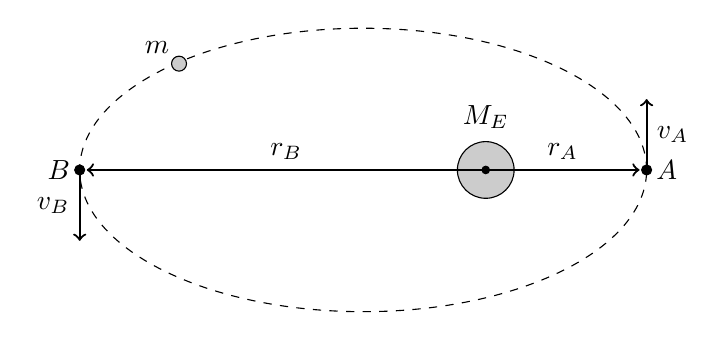
\begin{tikzpicture}[scale=0.9]
    %% Planet and orbit
    \draw[dashed] (0,0) circle (4cm and 2cm);
    %% Planet and satellite
    \draw[fill=white!80!black] (+1.73,0) circle (0.4cm) node[anchor=south,yshift=0.4cm] {$M_E$};
    \draw[fill=white!80!black] (150:3) circle (3pt) node[anchor=south east] {$m$};
    %% Orbital radius
    \draw[thick,<-] (-3.9,0) -- (1.73,0) node[pos=0.5,anchor=south] {$r_B$};
    \draw[thick,<-] (+3.9,0) -- (1.73,0) node[pos=0.5,anchor=south] {$r_A$};
    \draw[fill] (1.73,0) circle (1.5pt);
    %% Orbital points
    \draw[fill] (-4,0) circle (2pt) node[anchor=east] {$B$};
    \draw[thick,->] (-4,0) -- ++(270:1) node[pos=0.5,anchor=east] {$v_B$};
    \draw[fill] (+4,0) circle (2pt) node[anchor=west] {$A$};
    \draw[thick,->] (+4,0) -- ++(90:1) node[pos=0.5,anchor=west] {$v_A$};
\end{tikzpicture}
}

\element{njctl}{
\begin{question}{gravity-q19}
    A satellite of mass $m$ is traveling in an elliptical orbit about the Earth.
    At its furthest distance of $r_B$ its velocity is $v_B$.
    \begin{center}
        \njctlGravityQNineteen
    \end{center}
    What is its velocity at point $A$,
        which is a distance $r_A$ from the Earth's center?
    \begin{multicols}{2}
    \begin{choices}
      \correctchoice{$V_A = \dfrac{v_B r_B}{r_A}$}
        \wrongchoice{$V_A = \dfrac{r_B}{r_A}$}
        %% change v_r to v_B
        \wrongchoice{$V_A = \dfrac{m v_B r_B}{r_A}$}
        \wrongchoice{$V_A = \dfrac{v_B r_B}{m r_A}$}
        \wrongchoice{$V_A = \dfrac{v_B}{r_A}$}
    \end{choices}
    \end{multicols}
\end{question}
}

\element{njctl}{
\begin{question}{gravity-q20}
    A satellite orbiting around Jupiter at a distance $r$ from its center has a period of $T_1$.
    What would the period of an identical satellite orbiting at a distance $4r$ from Jupiter's center?
    \begin{multicols}{2}
    \begin{choices}
        \wrongchoice{$T_2 = \dfrac{T_1}{2}$}
        \wrongchoice{$T_2 = \dfrac{T_1}{4}$}
      \correctchoice{$T_2 = \dfrac{T_1}{8}$}
        \wrongchoice{$T_2 = 4T_1$}
        \wrongchoice{$T_2 = 8T_1$}
    \end{choices}
    \end{multicols}
\end{question}
}

\element{njctl}{
\begin{question}{gravity-q21}
    A satellite orbiting a planet at a distance of \SI{8e6}{\meter} from its center has a period of 16 hours.
    What would be the period of a satellite orbiting at a distance of \SI{2e6}{\meter} above the planet's center?
    \begin{multicols}{3}
    \begin{choices}
      \correctchoice{\SI{2}{\hour}}
        \wrongchoice{\SI{4}{\hour}}
        \wrongchoice{\SI{6}{\hour}}
        \wrongchoice{\SI{8}{\hour}}
        \wrongchoice{\SI{32}{\hour}}
    \end{choices}
    \end{multicols}
\end{question}
}

\element{njctl}{
\begin{question}{gravity-q22}
    A satellite is orbiting a planet at distance $r$ above its surface and has a period of $T$.
    What would the distance above the surface have to be in order for the period to become eight times greater?
    \begin{multicols}{2}
    \begin{choices}
        \wrongchoice{$R_{new}=\dfrac{R}{7}$}
        \wrongchoice{$R_{new}=\dfrac{R}{4}$}
        \wrongchoice{$R_{new}=R$}
        \wrongchoice{$R_{new}=4R$}
      \correctchoice{$R_{new}=7R$}
    \end{choices}
    \end{multicols}
\end{question}
}

\element{njctl}{
\begin{question}{gravity-q23}
    What is the total mechanical energy of a satellite of mass $m$ orbiting the Earth at a distance equal to 2 times the Earth's radius above its surface?
    \begin{multicols}{2}
    \begin{choices}
      \correctchoice{$E = -\dfrac{G m}{6 R_E}$}
        \wrongchoice{$E = -\dfrac{GM_E m}{4 R_E}$}
        \wrongchoice{$E = -\dfrac{GM_E m}{2 R_E}$}
        \wrongchoice{$E = -\dfrac{2GM_E m}{R_E}$}
        \wrongchoice{$E = -\dfrac{4GM_E m}{R_E}$}
    \end{choices}
    \end{multicols}
\end{question}
}

\element{njctl}{
\begin{question}{gravity-q24}
    Why does an astronaut appear to be weightless in a satellite orbiting the Earth?
    \begin{choices}
        \wrongchoice{The astronaut is unaffected by the Earth's gravitational pull at this distance}
        \wrongchoice{The Moon is exerting a force equal to and in the opposite direction of the force that the Earth is exerting. Therefore there is no net force acting on the astronaut}
        \wrongchoice{The astronaut is not accelerating}
      \correctchoice{The astronaut is in a constant state of free fall}
        \wrongchoice{When in space the astronaut has no mass}
    \end{choices}
\end{question}
}

\element{njctl}{
\begin{question}{gravity-q25}
    Suppose we drill a hole through the Earth along its diameter and drop a small mass $m$ down the hole.
    Assume that the Earth is not rotating and has a uniform density throughout its volume.
    The Earth's mass is $M_E$ and its radius is $R_E$.
    Let $r$ be the distance from the falling object to the center of the Earth.
    Which of the following describes the potential energy of the object as a function of distance $r$?
    \begin{multicols}{2}
    \begin{choices}
      \correctchoice{$E = -\dfrac{GM_E m r^2}{4 R_E^3}$}
        \wrongchoice{$E = -\dfrac{GM_E m r^2}{4 R_E^3}$}
        \wrongchoice{$E = -\dfrac{GM_E m r^2}{8 R_E^3}$}
        \wrongchoice{$E = -\dfrac{GM_E m r^4}{16 R_E^3}$}
        \wrongchoice{$E = -\dfrac{GM_E m r^3}{4 R_E^3}$}
    \end{choices}
    \end{multicols}
\end{question}
}

\element{njctl}{
\begin{question}{gravity-q26}
    For all gravitational problems involving $F= -GMm/r^2$,
        where do we consider the mass to be concentrated?
    \begin{choices}
        \wrongchoice{All of the mass is concentrated on the objects surface}
      \correctchoice{All of the mass is concentrated at the objects center}
        \wrongchoice{The mass is distributed throughout the object}
        \wrongchoice{The mass is considered to be concentrated halfway between the center and the surface}
        \wrongchoice{Its varies depending on the density of the planet}
    \end{choices}
\end{question}
}

\element{njctl}{
\begin{question}{gravity-q27}
    If a hole could be cut straight through the earth and a person dropped a ball of mass $m$ what path would the ball follow?
    \begin{choices}
        \wrongchoice{The ball will fall straight through the hole and come out the other side}
      \correctchoice{The ball will oscillate}
        \wrongchoice{The ball will stop once it reaches the center}
        \wrongchoice{The ball will never make it to the center}
        \wrongchoice{The ball will rebound as if it hit a floor and bounce back up to the person}
    \end{choices}
\end{question}
}

\element{njctl}{
\begin{question}{gravity-q28}
    A satellite is orbiting Earth in an elliptical orbit with radii $r_A$ and $r_B$.
    \begin{center}
        \njctlGravityQNineteen
    \end{center}
    If radius $r_B$ is five time of radius $r_A$,
        what is the ratio $v_B/v_A$ of the speed of the satellite at point $B$ to the speed at point $A$?
    \begin{multicols}{3}
    \begin{choices}
        \wrongchoice{$\dfrac{5}{1}$}
        \wrongchoice{$\dfrac{10}{1}$}
      \correctchoice{$\dfrac{1}{5}$}
        \wrongchoice{$\dfrac{1}{1}$}
        \wrongchoice{$\dfrac{1}{100}$}
    \end{choices}
    \end{multicols}
\end{question}
}

\element{njctl}{
\begin{question}{gravity-q29}
    A satellite is orbiting Earth in an elliptical orbit with radii $r_A$ and $r_B$.
    \begin{center}
        \njctlGravityQNineteen
    \end{center}
    If radius $r_B$ is five time of radius $r_A$,
        what is the ration $F_B/F_A$ of the force on the satellite at point $B$ to the force at point $A$?
    \begin{multicols}{3}
    \begin{choices}
        \wrongchoice{$\dfrac{5}{1}$}
        \wrongchoice{$\dfrac{10}{1}$}
        \wrongchoice{$\dfrac{1}{5}$}
      \correctchoice{$\dfrac{1}{1}$}
        \wrongchoice{$\dfrac{1}{100}$}
    \end{choices}
    \end{multicols}
\end{question}
}

\element{njctl}{
\begin{question}{gravity-q30}
    Two small spheres, each with a mass of \SI{1}{\kilo\gram},
        are separated by a distance of \SI{2}{\meter}.
    Which of the following is the order of magnitude of the gravitational force between the spheres?
    \begin{multicols}{3}
    \begin{choices}
        \wrongchoice{\SI{e-20}{\newton}}
        \wrongchoice{\SI{e-15}{\newton}}
      \correctchoice{\SI{e-11}{\newton}}
        \wrongchoice{\SI{e-7}{\newton}}
        \wrongchoice{\SI{e-3}{\newton}}
    \end{choices}
    \end{multicols}
\end{question}
}

%% Answer Key
%% 1.E 2.A 3.E 4.B 5.A 6.A 7.C 8.B 9.D 10.D 11.C 12.B 13.A 14.A 15.C 16.B 17.D 18.D 19.A 20.C 21.A 22.E 23.A 24.D 25.A 26.B 27.B 28.C 29.D 30.C


\endinput


